\documentclass{sig-alternate}
\usepackage[latin1]{inputenc}
\usepackage{graphicx}        % standard LaTeX graphics tool
\usepackage{url} 
\usepackage{subfigure}

\providecommand{\e}[1]{\ensuremath{\times 10^{#1}}}
\begin{document}
%
% --- Author Metadata here ---
\conferenceinfo{GECCO'14} {Vancouver, Canada}
\CopyrightYear{2014}
    \crdata{TBA}
    \clubpenalty=10000
    \widowpenalty = 10000



\title{A methodology to emerge literary plots using genetic algorithms} %FERGU: pensar un título que no de vergüenica, este me lo acabo de inventar 



\numberofauthors{2}
 \author{
 \alignauthor
 Anonymous\\
        \affaddr{Lost island}\\
        \affaddr{Unknown}\\
        \affaddr{Pacific Ocean}\\
        \email{jack,sawyer,hurley@lost.com}
 \alignauthor
 Anonymous\\
 \affaddr{Lost island}\\
 \affaddr{Unknown}\\
 \affaddr{Pacific Ocean}\\
 \email{locke@lost.com}
 }


\maketitle

%FERGU: TODOs
% 1) Pensar título
% 2) Escribir abstract
% 3) Quitar referencias a "second experiment"
% 4) Actualizar SOA
% 5) Contestar las preguntas de la intro en las conclusiones.

\begin{abstract}
%The creation of fictional stories is a very complex task that usually
%implies a creative process where the author has to combine characters,
%conflicts and plots to create an engaging narrative. This work
%presents a simulated environment with hundreds of characters that
%allows the study of coherent and interesting literary archetypes (or
%behaviours), plots and sub-plots. We will use this environment to
%perform a study about the number of profiles (parameters that define
%the personality of a character) needed to create two emergent scenes
%of archetypes: ``natality control'' and ``revenge''. A Genetic Algorithm (GA)
%will be used to find the fittest number of profiles and parameter
%configuration that enables the existence of the desired archetypes
%(played by the characters without their explicit knowledge). The
%results show that parametrizing this complex system is possible and
%that these kind of archetypes can emerge in the given environment.

%NUEVO ABSTRACT
Stories are not only painfully weaved by crafty writers in the
solitude of their studios; they also have to be produced massively for
non-playing characters in the videogame industry or tailored to
particular tastes in personalized stories. But the creation of
fictional stories is a very complex task that usually implies a
creative process where the author has to combine characters, 
conflicts and backstories to create an engaging narrative. This work
presents a methodology to generate cohesive and coherent literary
plots mainly for virtual environments using a Genetic Algorihm
(GA). This methodology helps the creation of the desired
environment and their parameters, but also of the parameters that model
the characters. Then, a genetic algorithm is used to establish the
parameter values that model the agents. Information of the simulation
of the environment can then be used to create the literary work. We
perform an implementation of this methodology using a specific
multi-agent system to validate our approach.

\end{abstract}

% A category with the (minimum) three required fields
\category{H.4}{Information Systems Applications}{Miscellaneous}
%A category including the fourth, optional field follows...
\category{G.1.6}{Mathematics of Computing}{NUMERICAL ANALYSIS}[Optimization]


%sures, performance measures
\terms{Algorithms}


\keywords{Genetic Algorithms, literature?}


%
%%%%%%%%%%%%%%%%%%%%%%%%%%%%%%%   INTRODUCTION   %%%%%%%%%%%%%%%%%%%%%%%%%%%%%%%
%
\section{Introduction}
\label{sec:intro}

In videogames, Non Player Characters (NPCs)  are a type of characters
that live in the game world to provide a more inmersive
experience and, in some cases, present a challenge to the human player. Modern RPGs (Role Playing Games), such as The
Witcher\texttrademark~or Skyrim\texttrademark~ include hundreds of NPC characters. The effort to create a good interactive fiction script is directly proportional to the number of these characters. That is the reason this kind of agents usually counts with limited behaviours, such as wandering in the villages, selling groceries or guarding the cities. Also, they usually offer scripted conversations, for example, to buy and sell objects to the player. In other cases they interact with the player depending of the player's behaviour: for example, if the player steals something a city guard would attack him.  However, these characters do not interact among them, only with the player, and their activities are only guided with this purpose. In a world with such a number of characters, their collective interactions could improve the gaming experience, leading to a richer and more inmersive world. For example, hungry inhabitants could become thieves, guards could pursuit the thieves, villagers could fell in love with others or different war alliances could emerge.


%FERGU: HABLAR DE LA METODOLOGÍA
These facts have motivated us to develop a ...

A set of probabilities and
states are associated to agents' actions, and these probabilities are
optimized by means of an Evolutionary Algorithm (EA) to match with a
specific literary archetype, defined by the fiction creator. The {\em
archetypes} are behaviours and patterns universally accepted and
present in the collective imaginary \cite{ArchetypesGarry05}, that
allows empathize  % mal escrito, y ¿existe empathize? - JJ
with the characters and immerse yourself in the story
(for example, the well-known {\em hero} archetype).
% Explica como caracterizas el arquetipo a partir de una serie de
% eventos en su historia personal y su relación con el resto de los
% personajes - JJ


To validate our methodology we also present a multi-agent system called
MADE (Massive Artificial Drama Engine) to model a self-organized
virtual world where their elements influences each other, following a
cause-effect behaviours in a coherent manner. This system needs to be
a suitable environment for the plot of a specific literary work, being
also interesting for the player/spectator. 

The aim of this work is to answer the following questions:

\begin{itemize}
 \item Is it possible to model a virtual environment inhabited by hundred of characters with interesting auto-generated behaviour based on literary archetypes?
 \item Could the personality of the agents be parametrized to obtain different behaviours?
 %\item How many profiles (groups of parameters that define a personality) are necessary to generate emergent quality sub-plots? %FERGU: quitada
 \item Could a Genetic Algorithm be used to find the fittest parameter values that allow the creation of quality sub-plots?
 \item Could be the obtained results of our methodology used to create a literary work? %FERGU: pregunta añadida que hay que contestar
\end{itemize}

%Estas preguntas son las que tienes que contestar en las
%conclusiones. Si no, el trabajo ha fallado - JJ2013 

In this paper we prove that EAs, together with a proper design of
literary patterns, can be used to find the parameters that promote the
generation of drama plots and sub-plots in a multi agent based
environment.\\

% pero ¿qué te da MADE? ¿Qué extraes de él? ¿La historia de los
% personajes? ¿El perfil de los mismos? Tenéis que dejar muy claro
% cuál es el PRODUCTO del algoritmo, porque si lo que tratas de hacer
% es un mundo en que los personajes sigan unos porcentajes
% determinados y eso es lo que obtienes, no tiene ninguna gracia - JJ

The rest of the work is structured as follows: after the state of the art, the developed system is presented in Section \ref{sec:made}. Then, the experiments conduced with the EA are shown (Sections \ref{sec:experimentalsetup} and \ref{sec:results}). Finally, conclusions and future works are discussed.

% -----------------------------------------------------------------------------
% SEC SOA

\section{State of the art}
\label{sec:soa}

% (JJ2013): Por cierto, acabo de ver esto: \cite{StoryTecGobel2008}.
% (Rubén): TODO

Auto-generated interactive fiction research is mainly focused in
methods to create the process of a story generation
\cite{nairat2011character}. Story generation can be divided in two
areas: interactive and non-interactive. In the first area, and
according to \cite{ReviewArinbjarnar09}, an Interactive Drama is
defined in a virtual world where the user has freedom to interact with
the NPCs and objects in a dramatically interesting experience,
different in each execution, and adapted to the interactions of the
user. % ¿Qué metodología usa cada uno? ¿En qué es mejor o peor que lo
      % que se va a hacer aquí?

The generation of interactive dramas can also be based in script
structure \cite{ArchitectureYoung04}, where each possibility in the
story must be previously defined, so there is a limited number of
possible plot combinations.

On the other side, in non-interactive plot generation systems the user
does not take control as the protagonist. For example, in the system
presented by Pizzi et al. \cite{pizzi2007interactive} the user can
interact with the characters, changing their emotions, but making the
user an spectator, rather than an actor. % La sección SoA es muy
                                % importante, porque enmarca el
                                % trabajo. Tenéis que hacerla más
                                % extensa y que tenga su propia
                                % narrativa - JJ

As opposed to those concepts, MADE is focused in Artificial Non
Interactive Drama, because its aim is the massive generation of plots
for secondary characters, to provide a context for the writer and the
player to perceive a virtual world as coherent, detailed and
enriched. The story generation (that is, the narrative) is not
addressed by MADE, but it has been studied in the systems presents in
the survey by Arinbjarnar et al. in \cite{ReviewArinbjarnar09}. 

% (JJ2013): Decir qué te hace suponer que esto va a ser una buena solución.
% (Rubén): TODO

Previous works define the plot as an emergence for the behaviour of the agents that follow a set of rules. In MADE, the agents' behaviour is product of its personality and the environment. That is, the agents does not follow the plot, but they generate the plot itself.


Furthermore, the previous works generate plots in worlds with a limited number of characters. This restriction does not exist in MADE, where the number of characters to create is unlimited.



Following the ideas of the work of Epstein and Axtell
\cite{epstein1996growing} an environment based in {\em Sugarscape} has
been developed with concepts such as food, metabolism and
vision. This environment uses the elements by Gershenson
\cite{gershenson2005general}: a virtual world, agents who are born, grow,

interact, reproduce and dead; resources (food), mediators, and
relations of rivalry (friction) and cooperation (synergy). The actions
of these agents are parametrized according the work of Nairat
\cite{nairat2011character}, based in the use of genetic algorithms to
obtain a plot (solution) where two characters interact in a creative way.

According to the taxonomy described by Togelius et al. \cite{Togelius2011}, the present work
with MADE can be seen has a \textit{procedural content generator} (\textit{PGC})
mainly related to \textit{optional content}, with \textit{stochastic generation}
and modelled as a \textit{generate-and-test} algorithm (search based) that
performs the optimizations of the process during the game development (\textit{offline}).

%The current experiment allows the definition of behaviour patterns (or
%archetypes, and using a weighted fitness function to measure
%the presence of the desired archetypes.



\section{Methodology}
\label{sec:methodology}

\subsection{Define agent}

\subsection{Define literary setting}

\subsection{Define GA}

\subsection{Instantiate parameters and execute}

\subsection{Convert results to literary language}



% -----------------------------------------------------------------------------
% SEC APPLY


\section{Applying the methodology}
\label{sec:applying}

\subsection{Agents in the MADE environment}
The MADE environment is a virtual place where different agents play their artificial lives. Its functions are:

\begin{itemize}
\item \textbf{Create an initial set of agents:} MADE environment
  initializes a set of just born orphan agents, each with a profile
  sequentially assigned.
% (JJ2013): Sequentially de qu� secuencia? - JJ2013
% (Rubén): TODO
 These agents must compete or collaborate in order to survive.
\item \textbf{Place agents in the map:} the environment has a squared map, formed by cells that can be occupied by one (and only one) agent. The environment allows the agents to discover and interact with other agents in the neighbourhood.
\item \textbf{Start and control the time:} after the creation of the initial set of agents, the MADE environment starts the timer, day by day until a maximum date is reached.
\item \textbf{Execute each agent during a time unit (a day):} In each iteration the list of agents is randomly reordered, and after that following the new order, each agent perform an iteration of its life-cycle, and the dead agents are removed from the grid.
\item \textbf{Perform as an external agent that changes th environment:} In each iteration in the MADE environment, food rations are placed in random cells. An agent only can eat if it is over a cell with a ration, so agents could move the other forcibly.
\item \textbf{Offer services to the agents:} MADE environment allow the agents to check which closer cells have food, are occupied, who agents are in a near position or which positions can be occupied.
\item \textbf{Decide the profile of the agents:} MADE allows the existence of different agent profiles, as previously said. A {\em profile} is a set of characteristics which governs the agent's behaviour.
\end{itemize}

The MADE environment can be configured by using the following parameters (and its values by default): Number of agents initially placed (15), map square grid dimension (10), number of rations randomly placed in the grid each day (10) and duration in virtual days of the  execution of the environment (1000). Those parameters can affect directly to the behaviour of the agents.

% (JJ2013): Usas un estilo demasiado conciso. Di qu� hace cada uno de esos
% par�metros, c�mo se meten (fichero de configuraci�n o como sea), por
% qu� se eligen esos y no otros, y los valores por defecto que has
% usado.

% (Rubén): por simplificar y reducir tamaño, pongo los valores por omisión

A MADE Agent lives in a MADE Environment, occupies a cell in the grid, moves around looking for food or mate and interacts with other agents.\\

%En un trabajo no se describe lo que se ha hecho, sino una
%metodología. Deberías justificar estos estados y las acciones. ¿Se
%pueden poner las que quieras? - JJ2013
The design of a MADE Agent has some restrictions:
\begin{itemize}
\item An array of parameters (probabilities represented as real numbers between 0 and 1) should be provided in its initialization. These parameters should be used by the agent in its day-by-day decisions.
\item Every action or event is subject to be logged for later analysis.
\item As a result of some iterations of the agent's day-based life cycle, the agent should present the behaviour of a \textit{living thing}, that is born, eats, grows, reacts, reproduces and dies.  
\end{itemize}

A very simple agent has been designed for this study: a virtual
rat, that models:
\begin{itemize}
\item Four states (be alive, be hungry, look for
mate and be pregnant) that represent internal situations that will lead the
agent to perform the actions described in the item bellow. % No se
                                % usan números Cambiar abajo - JJ
\item 7 actions (move, eat, attack, defend, escape,
find mate and have offspring) that lead to a basic instinctive animal
behaviour, very useful for this work since it can be the canvas of 
complex \textit{humanized} behaviour patterns.
\item parameters that define its characteristics and probabilities to
perform actions depending on the state.
\end{itemize}
It's important to remark that no ``feelings'' and no ``memory''
have been modelled in the MADE agent for this study. This is
illustrated in Figure~\ref{fig:madeAgent}.

\begin{figure*}
\begin{center}
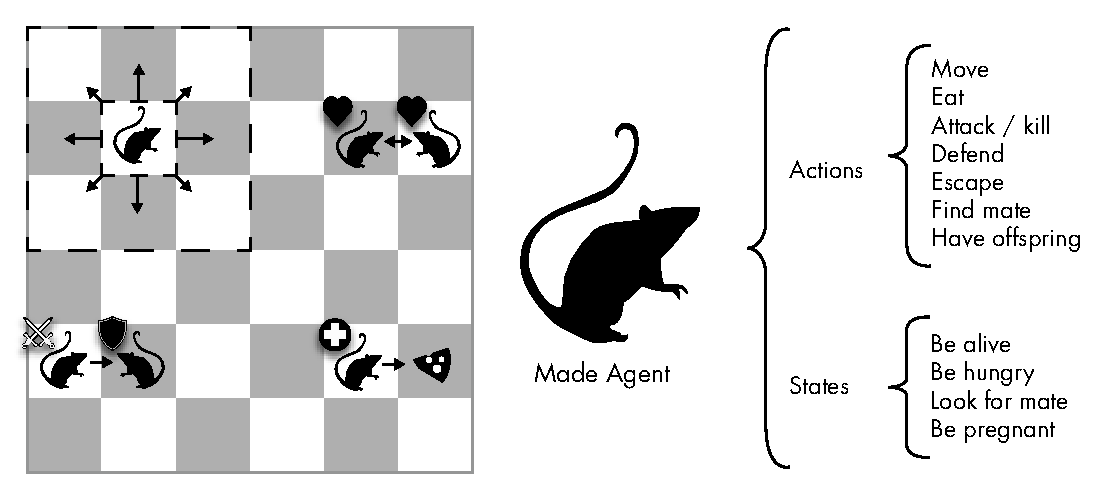
\includegraphics[scale=0.65]{img/MadeAgent.pdf}
\caption{Actions and states modelled in the MADE Agent.}
\label{fig:madeAgent}
\end{center}
\end{figure*}

\begin{figure*}
\begin{center}
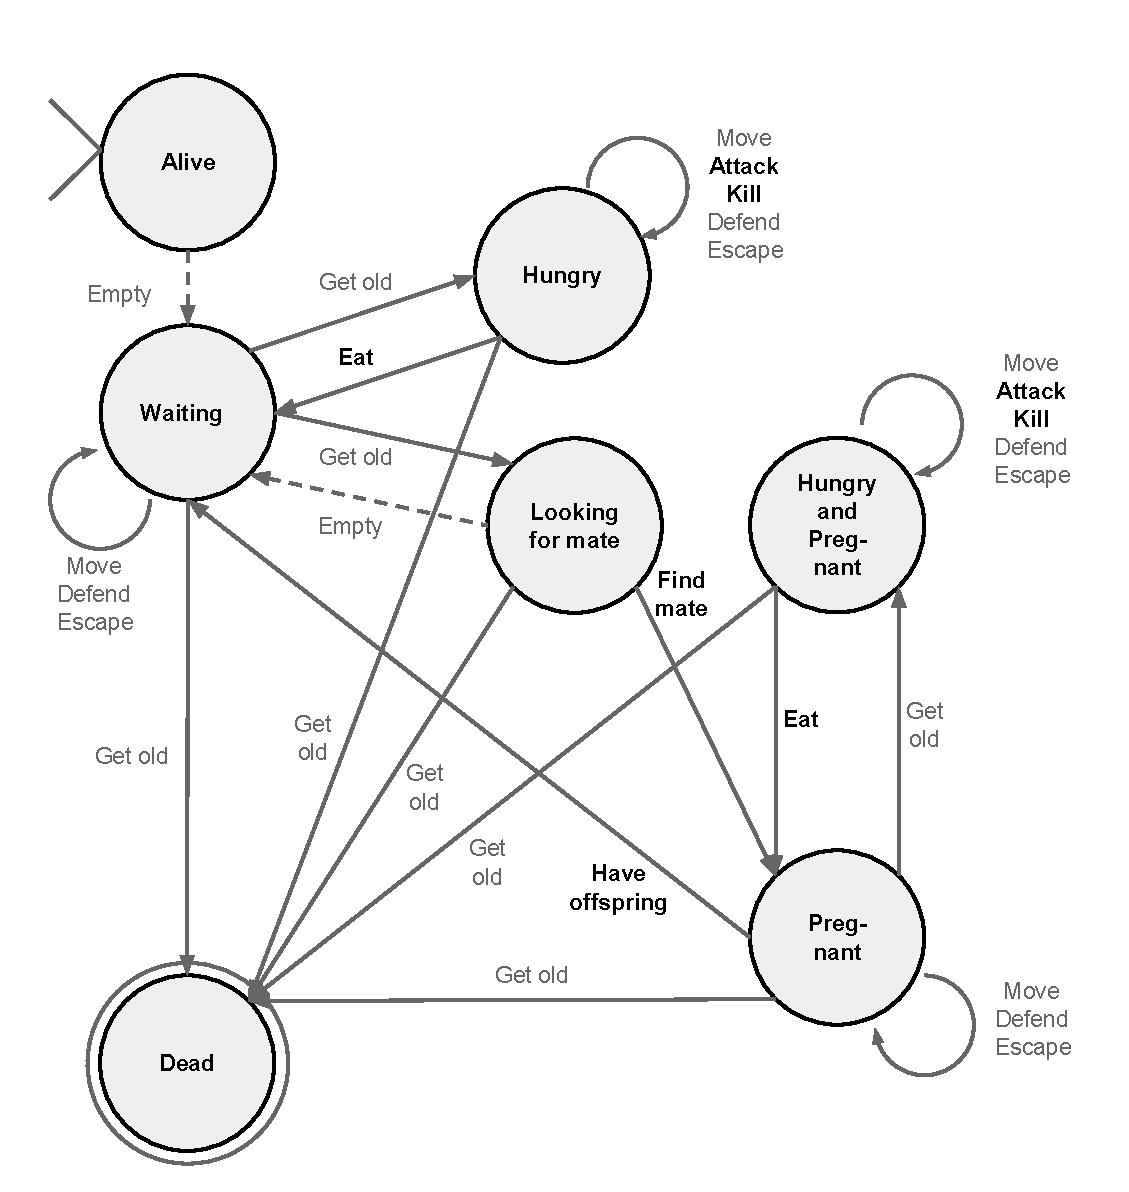
\includegraphics[scale=0.65]{img/fsm.pdf}
\caption{MADE Agent's finite state machine}
\label{fig:fsm}
\end{center}
\end{figure*}



%The life cycle of a MADE Agent illustrated in
%Figure~\ref{fig:lifecycle} represents on day in its life. 
Every
decision made by the agent is based on its state and its
characteristics (probabilities to perform different actions). % Los
                                % agentes son un FSM entonces, ¿no?
                                % Cita los papers en los que hablamos
                                % de FSM para Mario o Unreal, por ejemplo.
                                % ¿Esto es fijo? - JJ2013



% (Rubén): TODO ¿citar todas las características de un agente made?
% Sólo si hay hueco, creo
% No se ve nada y no aporta mucho. No uses notaci�n del programa, sino
% del algoritmo. Y mejor que lo contaras como un algoritmo usando el
% entorno algorithmic que este gr�fico. - JJ2013

% (Rubén): TODO No se cómo mejorarlo...

% Cámbialo por un algoritmo. Ocupa demasiado espacio y no se ve nada.
% O bien dibújalo como un autómata de estados finitos en vez de un
% diagrama de flujo. Un redondón por estado y flechas de transición -
% Además, me da la impresión de que estás mezclando estados de un
% bicho (pregnancy) con los de otro (a partir del nacimiento). Si es
% así, más que pregnancy deberías llamarlo "embryo" (y, sinceramente,
% no sé si merece la pena mencionarlo aquí y qué interés puede tener)
% JJ2013


The MADE Agent is created using twelve parameters, that define its
base features and probabilities to make the decisions presented in the
state diagram in Figure \ref{fig:fsm}. The execution of an
agent is dynamic, and depends on the internal probabilities and states
but also on the neighbourhood, and the map configuration. Even so, we
can say that these initial parameters define in some way the possible
situations where the agent could be involved.

The available source code of the MADE environment and the algorithms used in this experiment are publicly available in \url{http://ANONYMOUS} under a LGPL license.

\subsection{Definition of the literary setting}

 %The second scene is called
 This scene is called ``revenge'' and its goal is to model an individual complex memory
based behaviour between two characters.

The ``Revenge archetype'' scene, is performed to make more complex memory based behaviour emerge between two characters:  It tries to find what number of profiles and values are optimal to make \textit{revenge} archetype emerge in as many agents as possible after 1000 days.  An agent (a) will be considered as a \textit{avenger} if it has been attacked by other agent (b) and after that, in a moment in its life, it has satisfactory attacked the agent b, in revenge. The value of the days is set to 1000 because is a duration long enough to make the archetype emerge. 

\subsection{Definition of  the evolutionary algorithm}

We have defined the fitness function of this experiment as follows:
For each agent, if the agent's log matches the archetype, it adds 1 point to the fitness. Therefore, the goal is to recreate an environment where most ``avenger'' agents exist.

Thanks to the agents' logs, we can know every event (internal and
external) of their lives, and evaluate their interest or
adequacy to a specific literary setting.
                                % interest in
                                % what? Quieres decir si son
                                % interesantes? - JJ2013
In this work, we have implemented a method based in regular expressions with backreferences. The proposed technique puts annotations in every agent whose log matches a complex regular expression able to find emerging high level behaviours, not implemented in the life-cycle.

In this proposal, the parameters used to define an agent, mentioned in Section~\ref{sec:made}, are mapped into a chromosome, and a Genetic Algorithm is used to evolve the solution. The fitness function is expressed in terms of:

\begin{itemize}
\item \textbf{Regular expressions applied to the log of each agent in the environment:} An agent is tagged when a regular expression matches its log.
\item \textbf{A numeric function over the number of tagged agents for each archetype:} the fitness of the solution is incremented with the returning value.
\end{itemize}

Different number of profiles (from one to five) have been used to assign
% ¿Qué son los perfiles? No lo has definido en ningún sitio. Deberías
% ponerlo también en el abstract si es tan importante - JJ2013
% Sigue sin estar claro, ni qué relación hay entre perfiles,
% arquetipos, número d elos mismos ... igual un gráfico ayudaría. O un
% ejemplo - JJ
different parameters to different agents. If only one profile is used
in a run, all the agents are created with the same parameters, evolved
by the Genetic Algorithm. If more profiles are used, they are assigned
to the agents in order of appearance in a loop. Our assumption is that
some archetypes could emerge using one profile and other will need
more (those that require two clearly differentiated roles). It's
important to remark that the number of alleles of the chromosome are
multiplied by the number of profiles, so the convergence of the
solution could be affected by the number of profiles used. 

% Profile viene a ser las características o patrones que hacen que
% sepamos o podamos asociar una historia a un arquetipo, ¿correcto? No
% has hecho suficiente énfasis en esto y lo de los números queda un
% poco en el aire. Deberías introducirlo preguntándote eso: ¿cómo
% sabemos si un individuo corresponde a un arquetipo? Así introduces
% los perfiles, y luego hablas de que los perfiles se deben de hacer a
% mano, cuantos hacen falta... - JJ



\subsection{Instantiate parameters and execute}

For the experiments performed in this work, we have used the parameters shown in Table~\ref{fig:ga_parameters}. These values have been chosen empirically after several test runs.

\begin{table}
\begin{center}
\caption{Parametrization of the Genetic Algorithm}
\label{fig:ga_parameters}
\begin{tabular}{cc}%{p{3cm}p{7cm}}
\hline\noalign{\smallskip}
\noalign{\smallskip}
Parameter & Value \\
\hline
\noalign{\smallskip}
Codification & 12 alleles per profile\\
Fitness function & Average of 10 executions.\\
Natural selector & Original Rate: 0.9 \\
Crossover operator & Rate: 35\% \\
Mutation operator & Desired Rate: 12 \\
Stop condition & 100 executions\\
Generations & 30\\
Population size & 30 \\
\hline
\end{tabular}


\end{center}
\end{table}

\subsection{Analysis of the results}
The results of the experiment are shown in
Table~\ref{fig:exp2_30ex}. It shows the average of the best fitness
and the average population fitness at the end of each execution for
each configurations. Boxplots of the best fitness obtained are shown
in Figure \ref{fig:subfig2}. In this case, Krukal-Wallis and Wilcoxon
pairwise comparison shows significant differences among all
configuration (p-value $<<$ 0.05) except between P2 and P3
(p-value=0.3). Therefore, we can conclude that in this kind of global
archetype only a profile must be used for obtaining the best
results. This makes sense, because we are looking for one type of
local archetypes ({\em avenger}), so adding extra profiles leads to
different behaviours of the agents. 
% si vas a analizar los resultados, deberías mostrar tambień cómo
% cambia el mejor fitness y el intermedio, para que se pueda ver si el
% AG se hace bien o mal o regular. - JJ


\begin{table}
\begin{center}
\caption{Results for 30 executions of each configuration using 1 to 5 profiles in the experiment 2}
\label{fig:exp2_30ex}
\begin{tabular}{lllll}
\hline\noalign{\smallskip}
\parbox[t]{2cm}{Number of\\ profiles}
& \parbox[t]{3cm}{Best fitness\\(average) *}
& \parbox[t]{3cm}{Average\\fitness **} \\
\noalign{\smallskip}
\hline
\noalign{\smallskip}
1 & 495,513 $\pm$ 20,091 & 493,908 $\pm$ 19,884 \\
2 & 471,206 $\pm$ 24,550 & 469,361 $\pm$ 24,015 \\
3 & 455,42 $\pm$ 28,240 & 452,787 $\pm$ 29,438 \\
4 & 431,926 $\pm$ 31,682 & 428,206 $\pm$ 31,238 \\
5 & 411,24 $\pm$ 25,023 & 408,387 $\pm$ 23,829 \\
\hline
\end{tabular}
\\
\** Average of the best fitness at the end of each execution\\
\*** Average population fitness  at the end of each execution \\

\end{center}
\end{table}

\begin{figure}[htb]
\centering

%\subfigure[Experiment 1]{
%   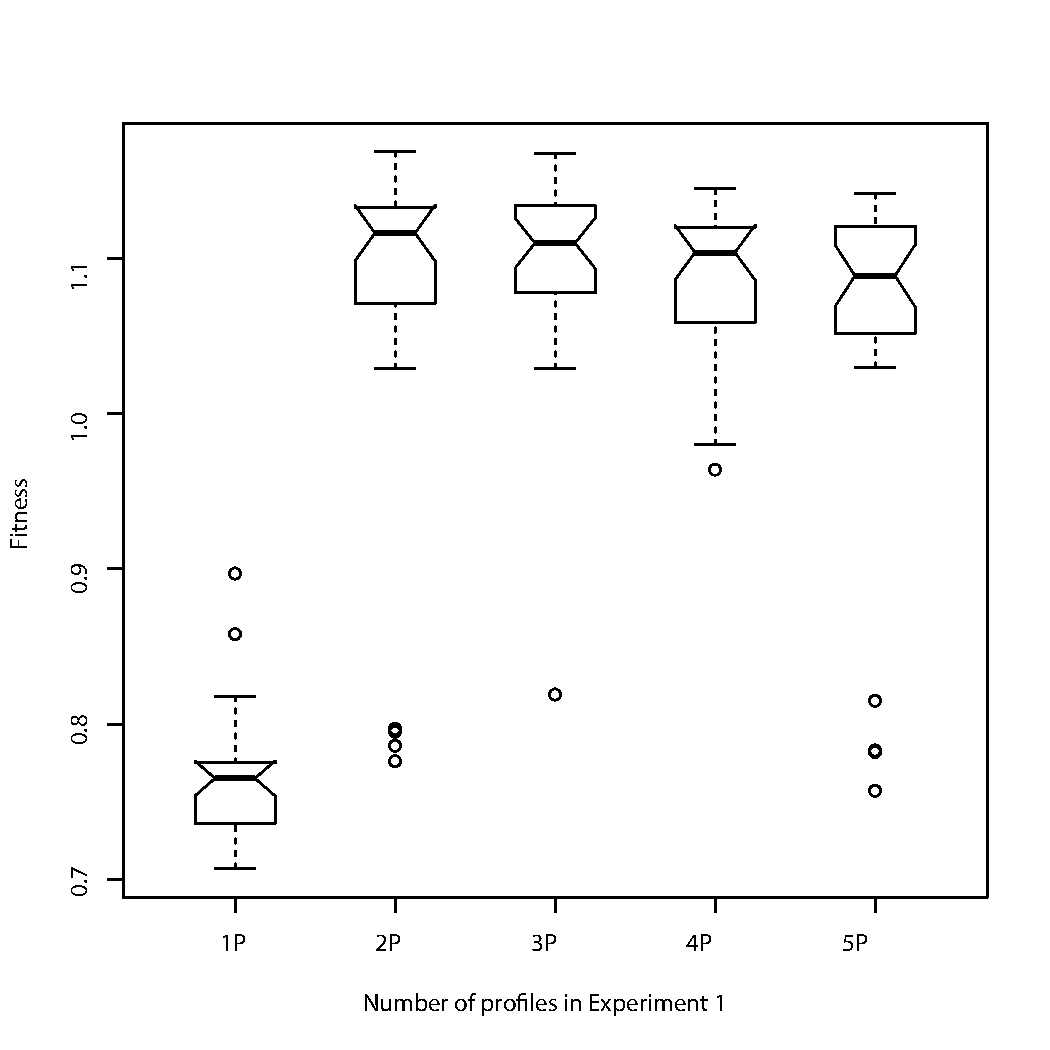
\includegraphics[width=13.5pc] {img/exp1_v2.pdf}
%   \label{fig:subfig1}
% }
%\subfigure[Experiment 2]{
   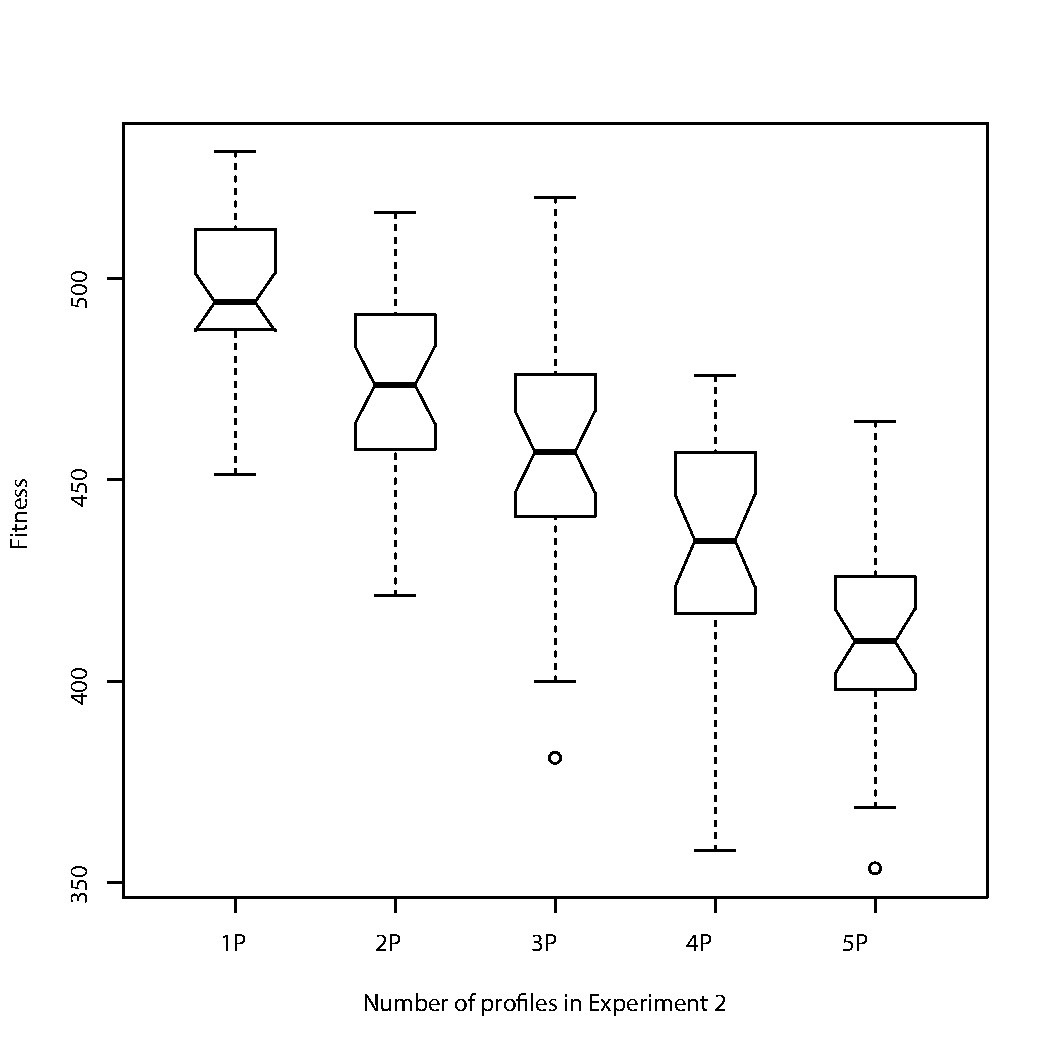
\includegraphics[width=13.5pc] {img/exp2_v2.pdf}
%   \label{fig:subfig2}
% }
\caption{Average fitness of the 30 best individuals for each configuration.}

\label{fig:graph}
\end{figure}

\begin{figure}[htb]
\centering

%\subfigure[Experiment 1]{
%   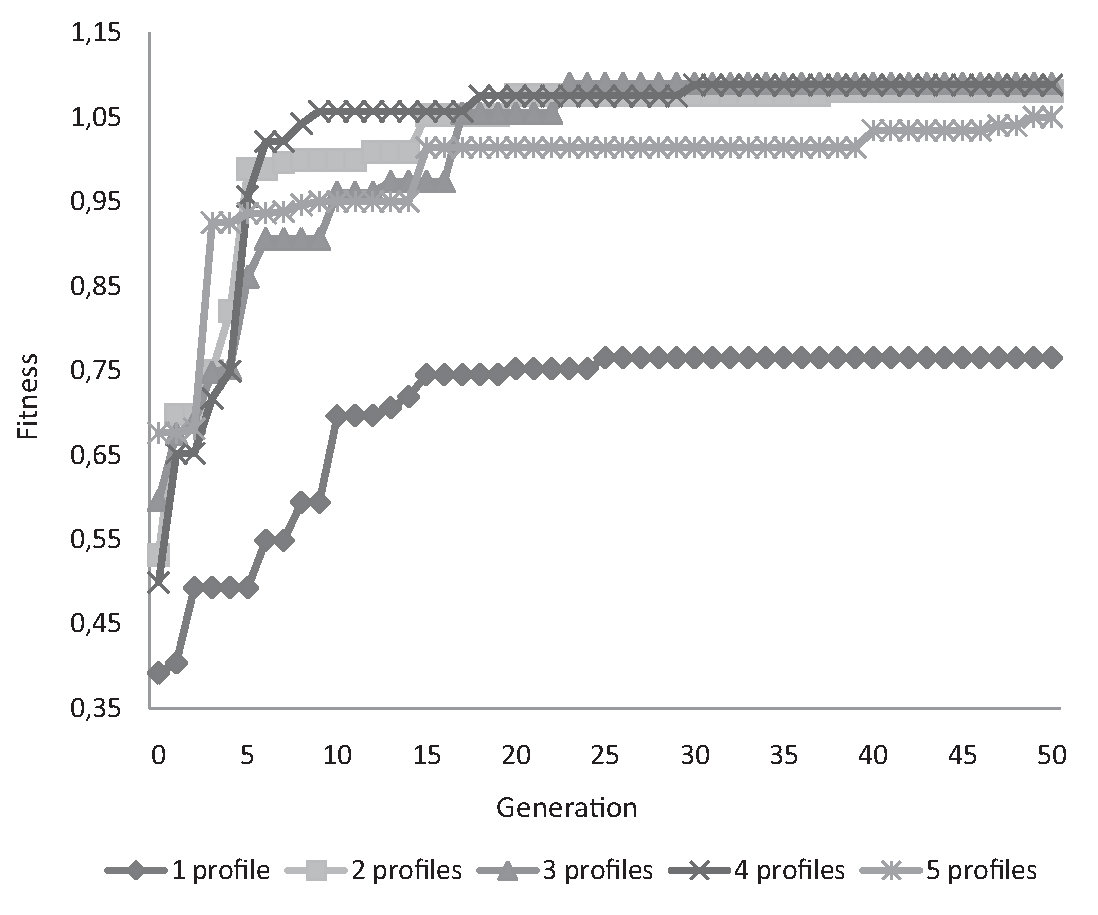
\includegraphics[width=13.5pc] {img/graph1_v2.pdf}
%   \label{fig:evo1}
% }
%\subfigure[Experiment 2]{
   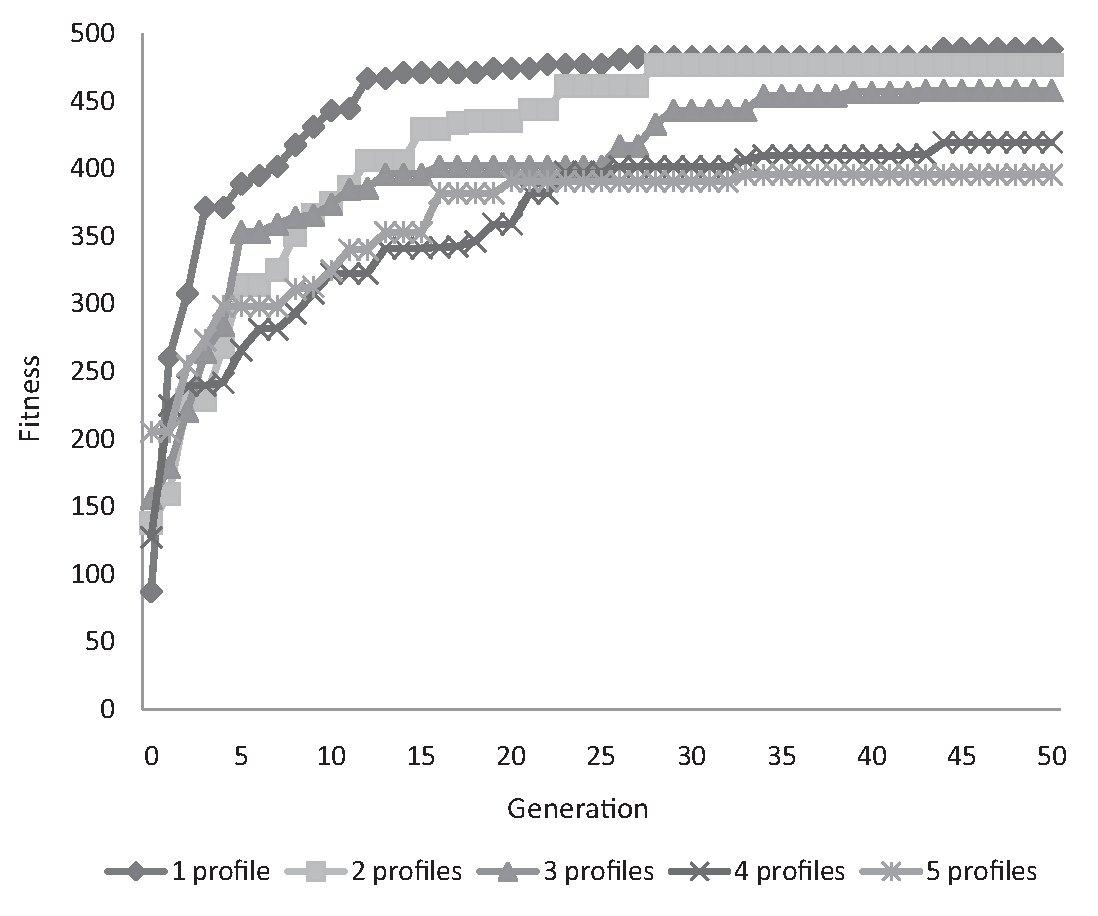
\includegraphics[width=13.5pc] {img/graph2_v2.pdf}
%   \label{fig:evo2}
% }
\caption{Example of the evolution of the best individual for the five
  profiles for each configuration.}
% ¿Qué hay que ver aquí? Comparar un número de perfiles con otro? - JJ2013

\label{fig:boxplots}
\end{figure}

\subsection{Convert results to literary language}

Every agent has a log that stores all the relevant events in its life
in a simple format. Each line of the log indicates the day, the event
in a short readable format and some extra information. Every agent's
log in the MADE Environment is coherent with all others' logs. Many
plots are being created, with a structured format that can be read by
game engines or natural language processors, but, given the simplicity
of the modelled agents, the stories could be seen by the reader as
non-interesting. This log can be used for evaluation. In the next
section we propose a method based on EA to let the author of a story
promote different behaviours in the MADE agents that could be seen as
literary archetypes (usually associated with human feelings and high
level cognitive and memory abilities) that can be used to model NPCs
in videogames (or be used in other creative areas). 
% ¿Aquí podrías hablar, o volver a hablar, de los perfiles, no? - JJ






% -----------------------------------------------------------------------------
% SEC EXPERIMENTALSETUP

\section{Experimental setup}
\label{sec:experimentalsetup}




% (JJ2013): Por qué has elegido estos experimentos y no otros? - JJ2013
% (Rubén): Done
% No del todo... lee abajo - JJ2013

%For this work, two sample groups of archetypes (or scenes)  have been
%chosen: % why only two and why _these_ two? - JJ2013
%The first one is called ``natality control'' and its goal is to model
%a global archetype (population growth) and four individual memory
%based archetypes (\textit{downtrodden}, \textit{helpless},
%\textit{warrior} and \textit{bad warrior}; these are related to their
%attack and defense behaviors).
                                % Defínelos, hombre o di
                                % algo de ellos, como "identified
                                % by". ¿Se supone que el lector
                                % sabe lo que son? ¿Qué tiene que ver
                                % la natalidad con los guerreros? - JJ2013



%The Experiment 1, ``Natality control'' scene, aggregates different sample archetypes where many factors must be taken into account.  It tries to find what number of profiles and values are optimal to:
%\begin{itemize}
%\item Ensure that, after 1000 virtual days, the alive population will be the 60\% of the total population. This is called a \textit{global archetype}.
%\item Emerge the \textit{downtrodden} archetype in the 22\% of the
%  population. An agent will be considered as a \textit{downtrodden} or
%  \textit{defender} if it has been attacked at least two times and has
%  defended the position.

%\item Emerge the \textit{warrior} archetype the 22\% of the population. An agent will be considered as a \textit{warrior} if it has satisfactory attacked at least five times.
%\item Emerge the \textit{helpless} archetype the 22\% of the population. An agent will be considered as a \textit{helpless}  if it has been attacked at least ten times and hasn't defended the position.
%\item Emerge the \textit{bad warrior} archetype the 22\% of the population. An agent will be considered as a \textit{bad warrior}  if it has unsatisfactory attacked at least ten times.
%\end{itemize}
%We have used the presented values to define this scene because, as our opinion, they model an interesting literary scene.

%To model this scenes we have defined the fitness function as follows:
%If the exact percentage of agents are tagged with one archetype defined, 1 point is added to the fitness. The maximum is therefore, 5 points. However, all the fitnesses use a normal distribution over the percentage of appearance. For example, for the first scene of archetypes (``growing population''), the maximum value (1) is obtained when the 60\% percent of the population is alive, and the normal distribution begins in the 30\% and ends in the 90\%. For the rest of the archetypes, 1 point is added if the 22'5\% of the population is tagged with each one of the archetypes, and each normal distribution begins in the 8\% and ends in the 30\%.

% (Rubén) TODO: ¿Es interesante poner las expresiones regulares?





 %AMOS, LA QUE TU QUIERAS, RUBEN (Fergu)

% (Rubén) TODO: ¿Es interesante poner las expresiones regulares?
% -----------------------------------------------------------------------------
% SEC RESULTS
\section{Results and discussion}
\label{sec:results}

%Table~\ref{fig:exp1_30ex} shows the average of the best fitness and the average population fitness at the end of each execution for each configuration: number of profiles from 1 (P1) to 5 (P5) in the experiment 1 (``natality control'').
%The evolution of the best fitness for each configuration is shown in Figure~\ref{fig:evo1}. We have performed a Kruskal-Wallis test for the best individuals fitness, obtaining differences among all the number of profiles (p-value $<<$0.05). As we suspected, it is clear that using one profile is not enough to emerge the desired archetype. However, the pairwise comparison using Wilcoxon does not find significant differences using more than 2 profiles. This can be explained because an agent could share more than one archetype at the same time.  A promising number of profiles could be 4, because their only lower outlier is not as distributed as the others. As can be seen in Figure \ref{fig:evo1} the evolution of the best fitness increases with all possible number of profiles, existing therefore an increase of the performance of the system.


%\begin{table}
%\begin{center}
%\caption{Results for 30 executions of each configuration using 1 to 5 profiles in the experiment 1}
%\label{fig:exp1_30ex}

%\begin{tabular}{lllll}
%\hline\noalign{\smallskip}
%\parbox[t]{2cm}{Number of\\ profiles}
%& \parbox[t]{3cm}{Best fitness\\ (average) *}
%& \parbox[t]{3cm}{Average\\ fitness **} \\
%\noalign{\smallskip}
%\hline
%\noalign{\smallskip}
%1 & 0,765 $\pm$ 0,037 & 0,761 $\pm$ 0,038 \\
%2 & 1,063 $\pm$ 0,115 & 1,059 $\pm$ 0,114 \\
%3 & 1,093 $\pm$ 0,063 & 1,091 $\pm$ 0,062 \\
%4 & 1,084 $\pm$ 0,048 & 1,082 $\pm$ 0,048 \\
%5 & 1,045 $\pm$ 0,110 & 1,041 $\pm$ 0,108 \\
%\hline
%\end{tabular}
%\\
%\** Average of the best fitness at the end of each execution\\
% Es decir, coges el mejor fitness de cada ejecucion (tendras 30 por cada
% numero de perfiles) y sacas la media
%\*** Average population fitness  at the end of each execution \\
% Igual, pero la media del fitness medio en la última generación.
% Vamos, lo copias de la hoja de cálculo, lo que está en negrita.
%\end{center}
%\end{table}




%\clearpage


% -----------------------------------------------------------------------------
% SEC CONCLUSIONS

%Lo más importante: responde a las preguntas que te has planteado? - JJ2013

\section{Conclusions}
\label{sec:conclusion}

%FERGU: REESCRIBIR ENTERA
%This work presents the result obtained by the MADE environment,
                                % no se presenta un entorno,
                                % se presenta los resultados obtenidos
                                % por él - JJ2013
                                % (Rubén:) ok
% a self-organized multi-agent
%system to model complex societies which can be used to study
%emergent behaviours for literary purposes; for example, to extract
%interesting plots for NPCs in videogames. %In this paper we have used
%the MADE environment to establish the number of profiles (sets of
%personality parameters) necessary to emerge two different global
%scenes: ``natality control'' and ``revenge'',
%which have been chosen because of their different nature: the first
%one consist in specific archetype rates (related to defense and attack
%behaviours of the agents) inside a global population rate, while the second one
%consist in maximizing the appearance of a memory based archetype, like the
%revenge (as previously said, memory hasn't been explicitly modelled in the
%agent).

We have used a
Genetic Algorithm to optimize the parameters of these profiles using
as a fitness a function that model the two desired global
archetypes. %Results show that in the first archetype the number of
%profiles must be at least two, because it is necessary that different
%behaviours (local archetypes) emerge. On the contrary, on the second
%experiment, using only one profile is the best configuration, because
%the purpose was to emerge only one archetype ({\em avenger}). If the
%number of profiles is increased worse results are obtained.

This implies that each scene or combination of desired archetypes for a given
environment can be mapped to a number of profiles that maximize the appearance
of these archetypes, and that the fittest number of profiles and its values can
be obtained by using Genetic Algorithms.  
Given a literary setting, an author of a story or a videogame could define 
different rates of archetypes or behaviour patterns and use the techniques described in
the present work to obtain the optimal profiles. The execution of the MADE Environment
using these profiles as input would produce a background (or set of characters' lives)
where the archetypes have emerged and have automatically created massive plots coherent
with the settings of the artwork.

In future works, more complex agents will be used, with different rules to be modelled. For example, we plan to model more human behaviours such as love or envy, to generate interesting plots such as wars, weddings, or family crimes. Different fitnesses will be used, for example, taking into account human opinions to establish the interestingness of a generated plot. Also, this system will be tested into an existent and well-known game, such as Skyrim\texttrademark, whose AI engine is publicly available for players and researchers.

% -----------------------------------------------------------------------------
% SEC ACKNOWLEGGEMENTS


\section{Acknowledgments}
This work has been supported in part %by FPU research grant AP2009-2942 and projects AmIVital (CENIT2007-1010), EvOrq (P08-TIC-03903), UGR PR-PP2011-5 and TIN2011-28627-C04-02.

%
% The following two commands are all you need in the
% initial runs of your .tex file to
% produce the bibliography for the citations in your paper.


%\bibliographystyle{abbrv} CAMBIAR!!!!!!
\bibliographystyle{plain}
\bibliography{made}  % sigproc.bib is the name of the Bibliography in this case


\end{document}